\documentclass[11pt,border=5pt]{standalone}
\usepackage{fontspec}
\setmainfont{cmunrm.otf}[BoldFont=cmunbx.otf,ItalicFont=cmunti.otf,BoldItalicFont=cmunbi.otf]
\usepackage{amsmath}
\usepackage{unicode-math}
\setmathfont{NewCMMath-Regular.otf}
\usepackage{tikz}
\usetikzlibrary{arrows.meta,patterns,angles,quotes}
\begin{document}
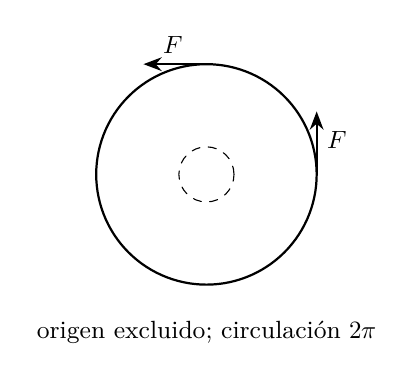
\begin{tikzpicture}[>=Stealth,font=\small,line cap=round,line join=round]
\draw[dashed] (0,0) circle (.35);
\draw[thick] plot coordinates {(1.40000,0.00000) (1.39808,0.07327) (1.39233,0.14634) (1.38276,0.21901) (1.36941,0.29108) (1.35230,0.36235) (1.33148,0.43262) (1.30701,0.50172) (1.27896,0.56943) (1.24741,0.63559) (1.21244,0.70000) (1.17414,0.76249) (1.13262,0.82290) (1.08800,0.88105) (1.04040,0.93678) (0.98995,0.98995) (0.93678,1.04040) (0.88105,1.08800) (0.82290,1.13262) (0.76249,1.17414) (0.70000,1.21244) (0.63559,1.24741) (0.56943,1.27896) (0.50172,1.30701) (0.43262,1.33148) (0.36235,1.35230) (0.29108,1.36941) (0.21901,1.38276) (0.14634,1.39233) (0.07327,1.39808) (0.00000,1.40000) (-0.07327,1.39808) (-0.14634,1.39233) (-0.21901,1.38276) (-0.29108,1.36941) (-0.36235,1.35230) (-0.43262,1.33148) (-0.50172,1.30701) (-0.56943,1.27896) (-0.63559,1.24741) (-0.70000,1.21244) (-0.76249,1.17414) (-0.82290,1.13262) (-0.88105,1.08800) (-0.93678,1.04040) (-0.98995,0.98995) (-1.04040,0.93678) (-1.08800,0.88105) (-1.13262,0.82290) (-1.17414,0.76249) (-1.21244,0.70000) (-1.24741,0.63559) (-1.27896,0.56943) (-1.30701,0.50172) (-1.33148,0.43262) (-1.35230,0.36235) (-1.36941,0.29108) (-1.38276,0.21901) (-1.39233,0.14634) (-1.39808,0.07327) (-1.40000,0.00000) (-1.39808,-0.07327) (-1.39233,-0.14634) (-1.38276,-0.21901) (-1.36941,-0.29108) (-1.35230,-0.36235) (-1.33148,-0.43262) (-1.30701,-0.50172) (-1.27896,-0.56943) (-1.24741,-0.63559) (-1.21244,-0.70000) (-1.17414,-0.76249) (-1.13262,-0.82290) (-1.08800,-0.88105) (-1.04040,-0.93678) (-0.98995,-0.98995) (-0.93678,-1.04040) (-0.88105,-1.08800) (-0.82290,-1.13262) (-0.76249,-1.17414) (-0.70000,-1.21244) (-0.63559,-1.24741) (-0.56943,-1.27896) (-0.50172,-1.30701) (-0.43262,-1.33148) (-0.36235,-1.35230) (-0.29108,-1.36941) (-0.21901,-1.38276) (-0.14634,-1.39233) (-0.07327,-1.39808) (-0.00000,-1.40000) (0.07327,-1.39808) (0.14634,-1.39233) (0.21901,-1.38276) (0.29108,-1.36941) (0.36235,-1.35230) (0.43262,-1.33148) (0.50172,-1.30701) (0.56943,-1.27896) (0.63559,-1.24741) (0.70000,-1.21244) (0.76249,-1.17414) (0.82290,-1.13262) (0.88105,-1.08800) (0.93678,-1.04040) (0.98995,-0.98995) (1.04040,-0.93678) (1.08800,-0.88105) (1.13262,-0.82290) (1.17414,-0.76249) (1.21244,-0.70000) (1.24741,-0.63559) (1.27896,-0.56943) (1.30701,-0.50172) (1.33148,-0.43262) (1.35230,-0.36235) (1.36941,-0.29108) (1.38276,-0.21901) (1.39233,-0.14634) (1.39808,-0.07327) (1.40000,-0.00000)};
\draw[->,thick] (1.4,0) -- (1.4,0.8) node[pos=0.55,right] {$F$};
\draw[->,thick] (0,1.4) -- (-0.8,1.4) node[pos=0.55,above] {$F$};
\node at (0,-2) {origen excluido; circulación $2\pi$};

\end{tikzpicture}
\end{document}
